\documentclass[12pt]{article}
\usepackage[utf8]{inputenc}
\usepackage{amsmath}
\usepackage{amsfonts}
\usepackage{amssymb}
\usepackage{amsthm}
\usepackage{graphicx}
\usepackage{natbib}
\bibliographystyle{ecol_let}
%\usepackage[colorinlistoftodos]{todonotes}
%\usepackage[style=ele]{biblatex}
\usepackage[mathlines]{lineno}

\usepackage{setspace}


%\usepackage{endfloat}
%\usepackage[default]{jasa_harvard}    % for formatting
%\usepackage{JASA_manu}


\begin{document}
\title{Important, Unique, Central: Species' Relevance in Food Webs}

\linenumbers

\maketitle

\begin{scriptsize}

\textbf{Authors:}
\begin{enumerate}
  \item Giulio Valentino Dalla Riva\\
	(corrisponding author)\\
	Biomathematics Research Centre\\
	School of Mathematics and Statistics\\
	University of Canterbury\\
	Christchurch, New Zealand.\\
	\textbf{E-mail:} gvd16@uclive.ac.nz
  \item	Carey E. Priebe\\
	Department of Applied Mathematics and Statistics\\
        Whiting School of Engineering\\
        Johns Hopkins University\\
	Baltimore, MD\\
	\textbf{E-mail:} cep@jhu.edu
\end{enumerate}

\begin{itemize}
\item \textbf{Running Title:} Important, Unique, Central
\item \textbf{Keywords:} Food Webs, Centrality, Functional Diversity, Evolutionary Distinctiveness, Random Graphs, Keystone Species, Community Ecology, Evolutionary Distinctiveness
\item \textbf{Type of Article:} Letters
\item \textbf{Abstract word count:} 147
\item \textbf{Manuscript word count:} 3222
\item \textbf{Number of figures:} 4
\item \textbf{Number of tables:} 1
\item \textbf{Number of references:} 46
\item GVDR designed the study and performed the analysis; GVDR and CEP developed and implemented the statical model; GVDR wrote the first draft of the manuscript and both authors contributed substantially to revisions.
\end{itemize}

\end{scriptsize}

\newpage

\doublespacing

%%%%%%%%%%%%%%%%

\begin{abstract}
	
Estimating the species' relative importance in an ecosystem is crucial to
preserve the planet's biodiversity. Unfortunately, the species' diversity makes
it hard to identify traits with a functional role across a large ecosystem.
Therefore, researchers have adopted a graph description of trophic interactions
in terms of food webs and graph-theoretical measures have been proposed to
estimate species' importance. However, these measures are often derived from
rigid models and their applicability to stochastic food webs is
limited. Here, we compute, from topological data, species' position in the food
web's abstract functional trait space and estimate the species' relative
importance for the food web's stability, their contribution to the food web's
functional diversity and their ecological uniqueness. We compare
the species' relevance as determined by our novel measures and six classic
measures. Finally, we explore the phylogenetic distribution of the species' relevance in
the Serengeti National Park food web.

\end{abstract}
%%%%%%%%%%%%%%%

\newpage
%%%%%%%%%%%%%%%%%%%%%%%%%%%%%%
%%%%%%%%%%    INTRO   %%%%%%%%%%%%%%
%%%%%%%%%%%%%%%%%%%%%%%%%%%%%%

\section{Introduction}\label{sec:intro}

The need for scientifically informed conservation policies boosted the attempts
to estimate species' relative importance in food webs: the graphs describing
the flows of energy between species in an ecosystem \citep{may2009food}. A
sound approach to assess a species' contribution to an ecosystem is based on the
concept of functional diversity. As summarised by
\citet*[pg. 742]{petchey2006functional} ``measuring functional diversity is about
measuring functional traits diversity, where functional traits are components
of an organism's phenotype that influence ecosystem level processes''. In this
context, the contribution of a species to the functional diversity of a food
web is captured by the traits diversity loss that we would observe after the removal
of that species \citep{villeger2008new, fontana2015individual}. However,
identifying suitable phenotypic traits and collecting all the necessary
data across a full food web is often ambitious. The tangled intricacy of food
webs, where there are often thousands of interactions between hundreds of plants and
animals, motivates the use of complex-network tools for solving ecological problems
\citep{proulx2005network}. Centrality measures---graph theoretical measures
developed in economic, social, technological and theoretical scenarios to
identify crucial nodes in a network \citep{newman2010networks}---have been
proposed to assess a species' centrality and to identify the species that play a
crucial role within an ecosystem
\citep{estrada2007characterization,lai2012centrality}.

The evolutionary distinctiveness of species (i.e., the amount of
\emph{exclusive} evolutionary information hinging on a species) is an
intrinsinc component of biodiversity \citep{mace2003preserving} and the
evolutionary diversity of species is used as a proxy for a species' functional
diversity \citep{winter2013phylogenetic}. Evolutionary diversity has been shown
to promote ecosystem stability \citep{cadotte2012phylogenetic}. Accordingly, it
has been argued that the evolutionary distinctiveness of species should be one
of the factors grounding conservation efforts
\citep{faith1992conservation,redding2006incorporating,isaac2007mammals}.
However, the exact relationship between the evolutionary and food-web
distinctiveness of a species is an open problem
\citep{gerhold2015phylogenetic,miranda2015congruence}.

The classic literature considers food webs to be discrete rigid objects
\citep{coulson2004skeletons}, in which an interaction between two
species (e.g., a predator and its prey) is either present (with a certain
weight) or absent; once an interaction is observed between individuals of two species,
at a particular point in time and space, that interaction is
extended uniformly at the species level. However, there is sound empirical and
theoretical evidence of stochastic variability in the structure of food webs,
depending on biotic and abiotic factors \citep{mullon2009minimal, poisot2015beyond}. This
motivates the distinction between a food web's backbone---its most statistically persistent
structure---and its fine wiring, which is more sensitive to contingent ecological
factors or stochastic noise \citep{grady2012robust, bellingeri2015food}. A robust ordering of species
based on their ecological relevance should not be too sensitive on
the fine wiring of a food web \citep{livi2011identifying}.

In another study \citep{dallariva2015exploring},  we introduced the random dot-product graph
model (RDPGs, see \citet{tang2013universally}) for food webs
and we showed that it offers an efficient approach to identifying food webs'
backbones. The RDPG model receives a classic binary description of a
food web (i.e., its adjacency matrix) and estimates the position of the species in
a continuous, metric space of \emph{abstract functional traits} determining
the species' interaction probabilities.  Each
species in a food web is associated with a pair of functional trait vectors: the
vulnerability functional trait vector, which describes a species as prey, and the
foraging functional trait vector, which describes a species as a predator. The
probability of observing an interaction from species $i$ to species $j$ (e.g.,
$j$ feeding on $i$) is given by the dot product of the vulnerability
functional traits of $i$ and the foraging functional traits of $j$.

Here, we show how the abstract functional trait space, estimated by the RDPG model,
offers a unified framework in which to assess species' importance, uniqueness
and diversity. We propose three measures, relying only on topological food-web data,
which can serve as proxies for measures based on phenotypic data. 

In the paper, we assess the  species' relative importance from their position in
the estimated abstract functional trait space for the Serengeti National Park's
food web \citep{baskerville2011spatial}, a highly resolved data set for which 
a comprehensive dated phylogeny is available. Building on the existing measures
of trophic similarity \citep{yodzis1999search,luczkovich2003defining,jordan2009trophic}, we define
the \emph{uniqueness} of a species' role within a food web as its
isolation (i.e., the average distance to all the other species) in the abstract
functional traits space estimated by the RDPG model. To measure the 
species' relative importance in a food web, we define a species' \emph{strain} as the
effect that removing that species has on the estimated abstract functional
trait space: for each focal species in the food web we measure the total
distance between the remaining species' positions in the abstract functional
trait space before and after the removal of the focal species. The strain of a species
captures a global effect at the whole food-web scale, rather than a local property of its interactions patterns.
Borrowing from the functional diversity literature, we estimate the functional diversity of a food web as the
volume of the convex hull enclosing all the species' abstract functional
traits. Accordingly, we define the contribution of a species to the functional
diversity of a food web as the loss in diversity caused by the removal of that
species.  Focussing on the vulnerability, on the foraging or both the
vulnerability and foraging abstract functional traits, we can assess a
species' relevance as prey, as a predator or as both predator and prey. We
distinguish amog the species' strain, uniqueness, and contribution to the
functional diversity as prey (\emph{outward} strain, uniqueness, and contribution to
the functional diversity), as a predator (\emph{inward} strain, uniqueness,
and contribution to the functional diversity) or as both a predator and prey
(\emph{total} strain, uniqueness, and contribution to the functional diversity).

We correlate these novel measures among each other as well as with six classic
network centrality measures, and we explore their distribution among the clades
present in the food web. In particular, we test whether the distribution of
ecological relevance among the tips of the Serengeti National Park food web's
phylogeny is compatible with an evolutionary model of traits evolution.
Finally, we examine the hypothesis that the species' ecological relevance and
evolutionary distinctiveness are indeed correlated.


%%%%%%%%%%%%%%%%%%%%%%%%%%%%%%
%%%%%%%%%% METHODS %%%%%%%%%%%%%%
%%%%%%%%%%%%%%%%%%%%%%%%%%%%%%

\section{Data and methods}

\paragraph{Food webs and phylogenies}
We focus our analysis on the Serengeti National Park food web as published
by \citet{baskerville2011spatial}. It is a large food web with 129
plants, 23 herbivores and 9 carnivores. Most of the links (507 out of 590) are between
herbivores and plants. The food web is less densely connected than other food webs, which is a
consequence of the higher than the usual taxonomic resolution of plants. In the
Supplementary Material, to support the general applicability of our framework, we
summarise the results for other three large food webs:
an independent compilation of the Serengeti National Park food web
\citep{de2011serengeti} and two marine food webs, one for the Caribbean Sea
\citep{opitz1996trophic} and one for the Antarctic Weddell Sea
\citep{jennings2002long}. The dated phylogenetic tree (available on-line) for
the species in the two Serengeti food webs has been compiled from molecular
data by De Zwaan \emph{et al.} \citep{dallariva2015exploring} (see the Supplementary
Material for more information). We approximated the real phylogeny for the
other webs via a cladogram obtained from the species' taxonomy as given by the
Integrated Taxonomic Information System (http://www.itis.gov; information
retrieved on 11 November 2014).

\subsection{Ecological and Evolutionary relevance}

\paragraph{Random dot product graphs}\label{subsec:method_rdpg}
Let $A$ be a food web including $S$ species.
Given a dimension $d$, under the RDPG model, each species $i$ in $A$
is associated to a pair of abstract functional trait vectors of dimension $d$.
The two vectors are the \emph{rank}-$d$ \emph{vulnerability} traits (or outward traits), which describes the
species as a prey or a resource, and the \emph{rank}-$d$ \emph{foraging} traits (or inward
traits), which describes the species as a predator or a consumer. The probability of observing an
interaction from species $i$ to species $j$ is given by the dot product of the
out traits of $i$ and the in traits of $j$. For an observed food web $A$, the
species'traits are estimated through a scaled, truncated, singular value decomposition
of the adjacency matrix of $A$ \citep{dallariva2015exploring} (see the
Supplementary Material for more details). 
The task of identifying a suitable range for the model's dimension is akin to a
dimensionality reduction problem, discussed for the Principal Component
Analysis scenario in \citet{jolliffe2002principal}. This can be solved
through the examination of the sequence of singular values of the adjacency matrix
of $A$. Here, we rely on the results of \citet{dallariva2015exploring}.

\paragraph{Strain}
The strain of species $i$ measures the effect that the removal of $i$ from the food web
has on the remaining species' abstract functional traits, as estimated from the
RDPG model. The effect is measured for species either as predators, as prey or as both. 
Let $X(A)$ be the matrix of either the inward, outward or total rank-$d$ abstract
functional traits (the last one being the matrixin  which the first $d$ columns are
given by the inward traits and the next $d$ columns are given by the outward traits).
We use $X(A)^{r(i)}$ to denote the matrix of the (inward, outward or total)
functional traits for all the species in the food web $A$ excpet $i$ (i.e.,
the matrix obtained by $X(A)$ removing the $i$th row).  The matrix
$X\left(A^{d(i)}\right)$ is the matrix of traits for the species in the food
web $A$ that has been computed after having dropped the species $i$ from the food web with
all its interactions (i.e., the matrix of traits computed after removing the $i$th row and column from $A$).
Both $X(A)^{r(i)}$ and $X\left(A^{d(i)}\right)$ are matrices with $S-1$ species (each species
in $A$ but $i$) and $d$ columns (the model's dimension). In $X(A)^{r(i)}$, the functional
traits are computed before removing $i$, in $X\left(A^{d(i)}\right)$ they are computed
after the removal event.
The (inward, outward or total) rank-$d$ strain of the species $i$ is the Procrustes distance
between $X(A)^{r(i)}$ and $X\left(A^{d(i)}\right)$. 

We are interested in the use of RDPG-based measures to value species in a way that
is robust to model parameters. Therefore, we tested whether the species' ordering by strain
was sensitive to the choice of model dimensionality and performed a pairwise correlation test for each pair of
dimensions in the range $\left[1, \dots, 15 \right]$. Notice that the latter upper
range limit is much greater than the suitable upper bound for model dimensionality found
in \citet{dallariva2015exploring}.

\paragraph{Uniqueness}
We define the rank-$d$ \emph{uniqueness} of a species in a food web, either as
a predator, prey or both, as the average of its
Euclidean distance to every other species in the $d$-dimensional (inward, outward or total)
abstract functional trait space.

\paragraph{Diversity}
The volume of the convex hull of a community of species in the traits space is a
proxy for its functional diversity \citep{villeger2008new}. Here, we define the
contribution of species $i$ to a food web's abstract functional diversity as
the difference in volume between the convex hull of the species traits, in the
(inward, outward or total) abstract functional space, before and after species $i$ is removed (i.e, the
difference between the volume of the convex hull of $X(A)$ and $X(A)^{r(i)}$).

\paragraph{Keystone centralities} We assessed the keystone centrality of a
species $i$ in a food web $A$ by using six different (topological) network measures following
\citet{estrada2007characterization}: degree centrality, betweenness centrality \citep{brandes2001faster},
closeness centrality  \citep{freeman1979centrality}, eigenvector centrality
\citep{bonacich2001eigenvector}, information centrality
\citep{stephenson1989rethinking}, subgraph centrality
\citep{estrada2005subgraph}. All the measures we introduce and the six examined by \citet{estrada2007characterization}
are computable for unweighted food webs (weighted extensions are definable, but we do not address
them here). More details about the above theoretical measures
can be found in \citep{jordan2009trophic}. We chose these measures as their evaluation does
not rely on morphological trait data nor on interaction weights.

\paragraph{Phylogenetic diversity}
Phylogenetic diversity \citep{hartmann2007phylogenetic} offers an alternative
way to evaluate the diversity of a community of species. The phylogenetic
diversity of an evolutionary tree is the total sum of branch lengths in that
phylogeny. This concept has been applied in the prioritisation of species
for conservation purposes \citep{faith1992conservation,mace2003preserving}.  We
each estimated species' evolutionary distinctiveness by
measuring its fair proportion value \citep{isaac2007mammals}, equal
splits value \citep{redding2006incorporating} and the length of the terminal
phylogenetic branch leading to that species, following \citet{faye2015valuing}.
The fair proportion and equal split scores attempt to apportion the total
evolutionary  history of a phylogeny among the extant species. These three
measure are known to be positively correlated.

More details on the implementation of these diversity measures can be found in the Supplementary
Material.

\subsection{Comparative analysis}
Because of their shared evolutionary histories, we would expect to observe more similar
traits for more closely related species, a concept recognised at least
since the work of \citet{felsenstein1985phylogenies}.  The evolutionary
dependency of species arises the statical issue of controlling and correcting
for the phylogenetic covariation structure of the observed species' traits.
To select the appropriate evolutionary model, we compute the relative Akaike information criterion
corrected for finite sample size (AICc, see \citet{hurvich1989regression})
of four distinct models \citep{garamszegi2014multimodel}. We
consider an uncorrelated null model, a Brownian motion model
\citep{felsenstein1985phylogenies}, a Brownian motion with attraction toward an
optimum (Ornstein--Uhlenbeck) model \citep{hansen1997stabilizing} and a model with early
eurst of differentiation \citep{harmon2010early}.
We test for linear correlations among the (inward, outward and total) novel measures (of strain,
uniqueness, and contribution to functional diversity) and among (inward, outward and total)
strain and uniqueness and the six keystone centralities. To do so, we use generalised
least square regression techniques, either controlling for the appropriate
phylogenetic covariance structure associated with the evolution model with the highest
AICc weight, or under the null evolutionary model.

%%%%%%%%%%%%%%%%%%%%%%%%%%%%%%
%%%%%%%%%%  RESULTS  %%%%%%%%%%%%%%
%%%%%%%%%%%%%%%%%%%%%%%%%%%%%%

\section{Results}

We computed the species strain for $d \in \left[ 1, \dots,  15 \right]$ (Fig. 1
a). In \citep{dallariva2015exploring} we estimated a suitable model dimension $d = 3$
for the Serengeti National Park food web.  The species'
strain (model dimension $d = 3$) has an average value of $0.032$ and a variance of $0.017$;
a small number of species have a high strain (Fig. 1b). The
three species with the highest strain are all in the Afrotheria clade (and represent
the totality of that clade in the food web). These are \emph{Procavia
capensis} (rock hyrax, strain $= 1.316$), \emph{Heterohyrax
brucei} (yellow-spotted rock hyrax, strain $= 0.884$) and
\emph{Loxodonta africana} (the African bush elephant, strain
$= 0.317$). The ordering of species based on their strain is robust to the
choice of model dimension, in the range $d \in \left[ 1, \dots,  15 \right]$
(Fig. 1 c). Every pairwise ordering correlation in the analysed
interval is significant at $p < 0.01$ (this result is also confirmed
by the analysis of the independent assembly of the Serengeti National Park food
XXX web by \cite{de2011serengeti}; see the Supplementary Material).

The Afrotheria are also characterized by high uniqueness in terms of their
mean distance to the other species in the abstract functional trait space. The observation can
be extended the species' phylogeny, noticing that the two measures are non-uniformly
distributed among the tips of the phylogenetic tree (Fig. 2 a). There is also support
for an Ornstein--Uhlenbeck (Brownian motion with attraction toward
an optimum) model of evolution for both strain and uniqueness (Fig. 2 b). The
correlation between species' (outward and total) strain and uniqueness is
significant at $p < 0.01$, while the species' inward strain and
uniqueness are not consistently correlated for $d > 4$ (Fig. 3 a). 
The computation of the species' contribution to the abstract functional
diversity for $d > 4$ (species as both predators and
prey) and $d > 7$ (species as either predators or prey) was not possible because
of software limitations. However, in the feasible range of $d$, the species' total strain is
significantly positively correlated with both the species' total uniqueness
and their contribution to the total functional diversity (Fig. 3 b). The
correlations for the partial (either inward or outward) measures are not consistently
significant and depend on the measure considered.

The strain and mean distance of species in the Serengeti National Park are, in
general, positively correlated with the common keystone centralities (Fig. 4).
The significance and strength of the correlations depend on the particular
combination of the centrality measure, the  model dimension and the functional space
considered (either inward, outward or total). We observed the most consistent
correlations with the Betweenness, Subgraph and Degree centralities.
The correlation results are qualitatively confirmed by performing the regression analysis
either accounting for or ignoring the species' phylogenetic covariance structure. Hence
the correlations hold whether or not we consider the phylogenetic structure
of the food web. This general agreement between our novel measures and the common graph-theoretical
indices used to identify keystone species supports the applicability of the RDPG model for food
webs. 

Although there are species with both high phylogenetic distinctiveness and high
strain or uniqueness (Tab. 1), we did not detect any significant linear
correlation between the species' evolutionary and ecological relevance measures.

%%%%%%%%%%%%%%%%%%%%%%%%%%%%%%
%%%%%%%% CONCLUSION %%%%%%%%%%%%%%
%%%%%%%%%%%%%%%%%%%%%%%%%%%%%%

 \section{Discussion}

For each species in the food web, we researched its position in the (inwad, outward and
total) abstract functional trait space for $d \in \left[ 1, \dots, 15\right]$
and computed three measures of ecological relevance (strain, uniqueness and
contribution to functional diversity). We verified that species' ordering
based on the measures we introduced is robust to the choice of the model's dimension
$d$. The RDPG model for food webs allows us to distinguish between the low-dimensional,
stochastic backbone of a food web and its fine wiring. The
stochastic backbone is robust to food web variability and to misspecifications
of the food web structure, such as a missed observation of an interaction or
an erroneous recording.  Being based on the estimated (low-dimensional)
structural food-web backbone, the measures we introduced are themselves robust
to the variability of complex food webs. Other classic measures of trophic
uniqueness \citep{yodzis1999search,luczkovich2003defining,jordan2009trophic} do
not make this distinction.

The RDPG model allows us to estimate the abstract functional
diversity of a food web by relying solely on topological data. It remains to
be ascertained whether there is a correspondence between the classic
morphological functional diversity and our novel concept of abstract
functional diversity. If verified, the abstract functional diversity may serve
to estimate the (classic) functional diversity without the burden of
identifying suitable phenotypic traits with a functional role across all the
species in a food web---an ambitious task, given species' heterogeneity.  Our results appear to point toward a positive answer. The
range of suitable abstract space dimensions estimated under the RDPG model (not
higher than five, see \citep{dallariva2015exploring}), is in good accordance
with the number of (classic) functional traits that  \citet{maire2015many}
estimated for an optimal (classic) functional diversity analysis.

We showed that a species' abstract functional trait uniqueness is positively
correlated with its classic centrality in the Serengeti National Park food web.
The result was also confirmed for the Weddell Sea food web
\citep{jennings2002long}, the Caribbean Sea food web \citep{opitz1996trophic}
and the independent compilation of the Serengeti National Park food web by \citet{de2011serengeti}
(see the Supplementary Material for details).
A positive correlation between classic functional uniqueness, \emph{sensu}
\citet{yodzis1999search},  and the degree centrality---the number of trophic
interactions---has already been established by \citet{petchey2008trophically}.  The
result is even more interesting if read in comparison with the negative
correlation found by \citet{lai2012centrality} between the classic centralities
and the trophic uniqueness of a species \emph{sensu} \citet{luczkovich2003defining}
and \citet{jordan2009trophic}.  Further comparative analyses are therefore
needed to explain this difference and explore the relationship between the abstract
functional uniqueness of a species and its trophic uniqueness as otherwise
defined. Similarly, a species' strain  is positively correlated with its
classic centrality and that a species' uniqueness predicts its strain. In
addition, both strain and uniqueness are are positively correlated
with a species' contribution to the abstract functional diversity of the food
web. \citet{petchey2008trophically} have shown that trophically unique species
are exposed to a higher risk of secondary extinction, highlighting their
fragility. Conversely, the correlation between uniqueness and strain supports
the notion that food webs are particularly fragile to the extinction of
functionally unique species, as already suggested by \citet{o2010loss}.

The ecological relevance---strain and uniqueness---of the species in the Serengeti food web
is not uniformly distributed across the phylogeny (in fact, it is compatible with the distribution
we would expect under a Ornstein-Uhlenbeck model of evolution). We did not detect a
significant correlation between the species' ecological relevance and their
evolutionary distinctiveness. However, a small number of species have both
high ecological relevance and high evolutionary distinctiveness. This is the
case in the Afrotheria clade (i.e., the African elephants and two hyrax species).
The peculiarity of the Afrotheria clade has already been suggested by \citet{baskerville2011spatial}
on the basis of the particularity of the hyrax's trophic role.
Our results confirms the importance of considering both ecological and evolutionary factors
in the evaluation of species for conservation purposes.

%%%%%%%%%%%%%%%%%%%%%%%%%%%%%%
%%%%%%%%%%%  BIBLIO  %%%%%%%%%%%%%%
%%%%%%%%%%%%%%%%%%%%%%%%%%%%%%

\begin{small}
	\bibliography{asgefw}
\end{small}


%%%%%%%%%%%%%%%%%%%%%%%%%%%%%%
%%%%%%%%%   FIG & TAB  %%%%%%%%%%%%%%
%%%%%%%%%%%%%%%%%%%%%%%%%%%%%%
\newpage
\appendix
\newpage
\small
\subsection*{Figure 1}
The distribution of species' strain in the Serengeti National Park food web
\citep{baskerville2011spatial}.
(a) The line trace strain of each species ($\mbox{\texttt{Log}}_{10}$ transformed) along
an increasing model dimension ($d \in \left[ 1, \dots , 15\right]$). The strain
has been computed for species as both predators and prey.
(b) A cross-section of (a) for $d  = 3$ (corresponding to the suitable model dimension we
identified in \citep{dallariva2015exploring}).
(c) Pearson product-moment correlation coefficients for the species ordering induced by the
species' total strain across the model dimensions $d \in \left[ 1, \dots , 15\right]$.
The ordering is robust to the choice of the model dimension $d$: the Pearson's \textit{r} is consistently
above 0.5 (and all the pairwise correlations are significant at $p < 0.01$).

\begin{figure}[h!]
 \centering
 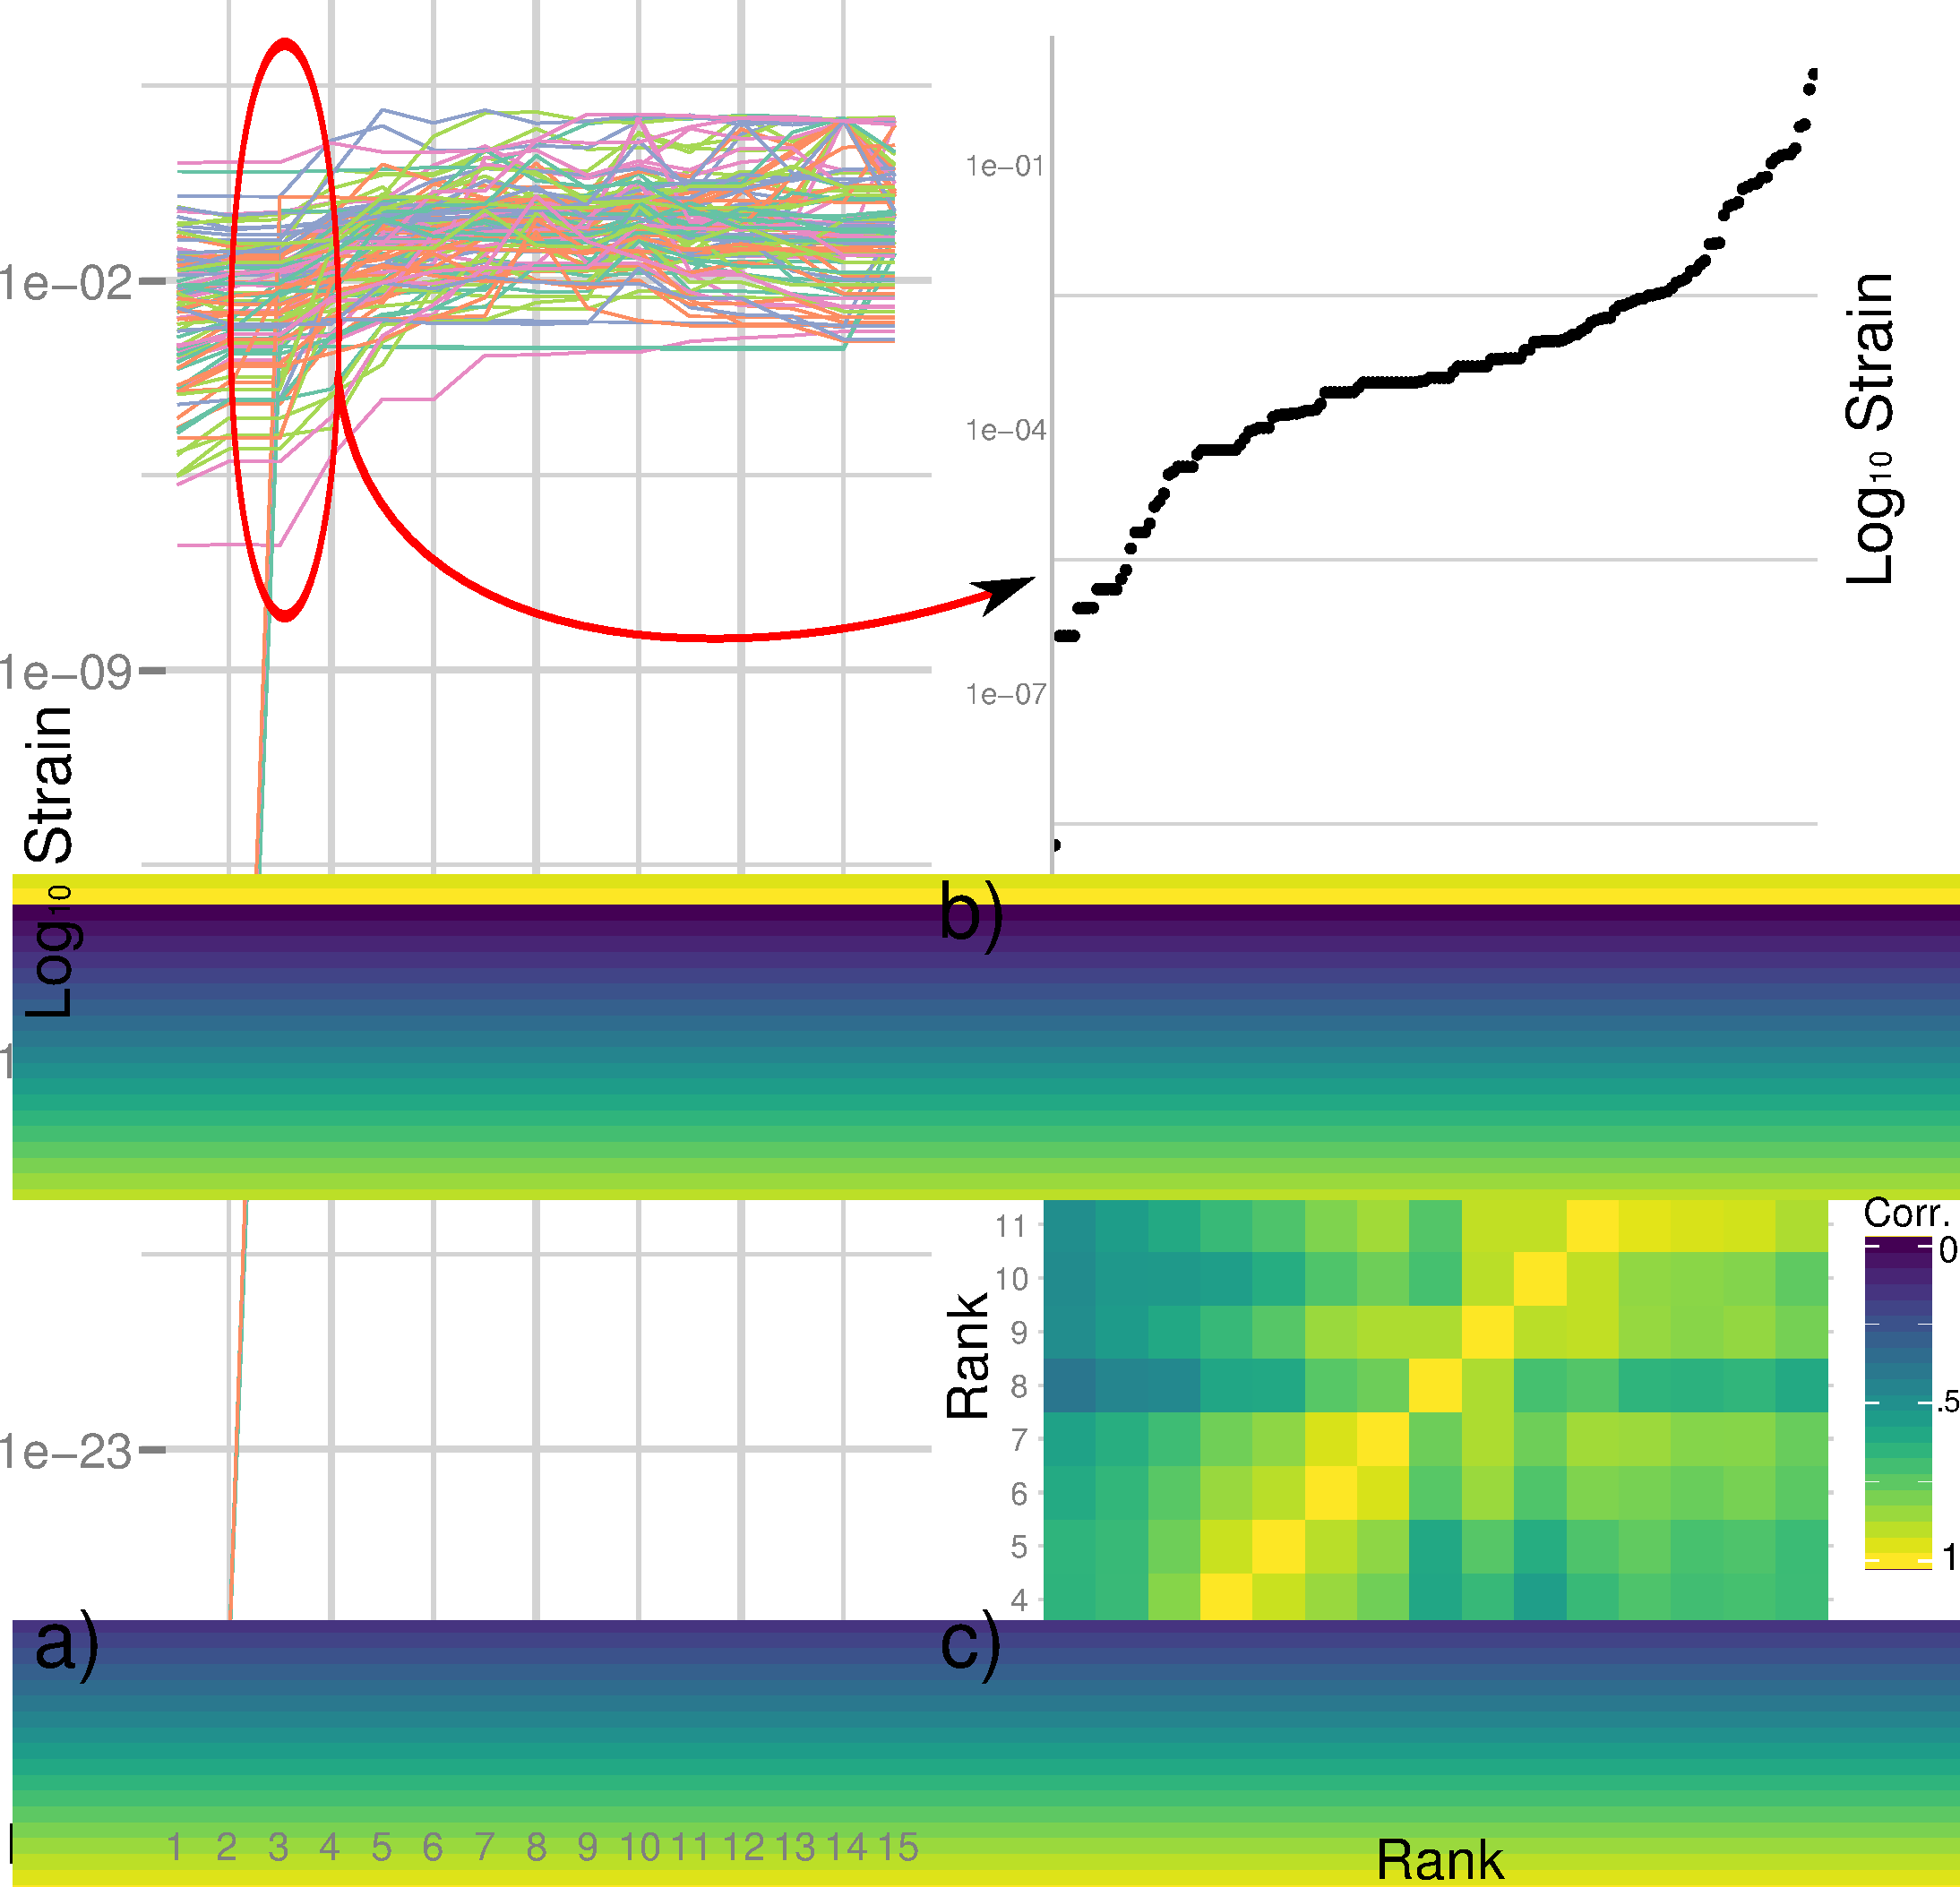
\includegraphics[width=0.8\textwidth]{./Images/Figure_1.pdf}
\end{figure}
\newpage

\subsection*{Figure 2}
(a) Distribution of rank-$3$ species' strain and uniqueness in the phylogeny
(lighter yellow for lower values; darker blue for higher values) for species as both
predators and prey (all). The silhouettes (from phylopic.org) mark the corresponding clades:
Afrotheria (hyraxes and elephants) are the species with the highest strain and uniqueness.
(b) Akaike Information Criterion (corrected for sample size) weights for four models of species'
(inward, outward and total) strain and uniqueness evolution:
uncorrelated, Z; Brownian motion, B \citep{felsenstein1985phylogenies};
Ornstein-Uhlenbeck, OU \citep{hansen1997stabilizing}; Early Burst, E
\citep{harmon2010early}. The data consistently supports an OU model, except
for the low-dimension strain evolution, in which there is also good support for the B model.

\begin{figure}[h!]
 \centering
 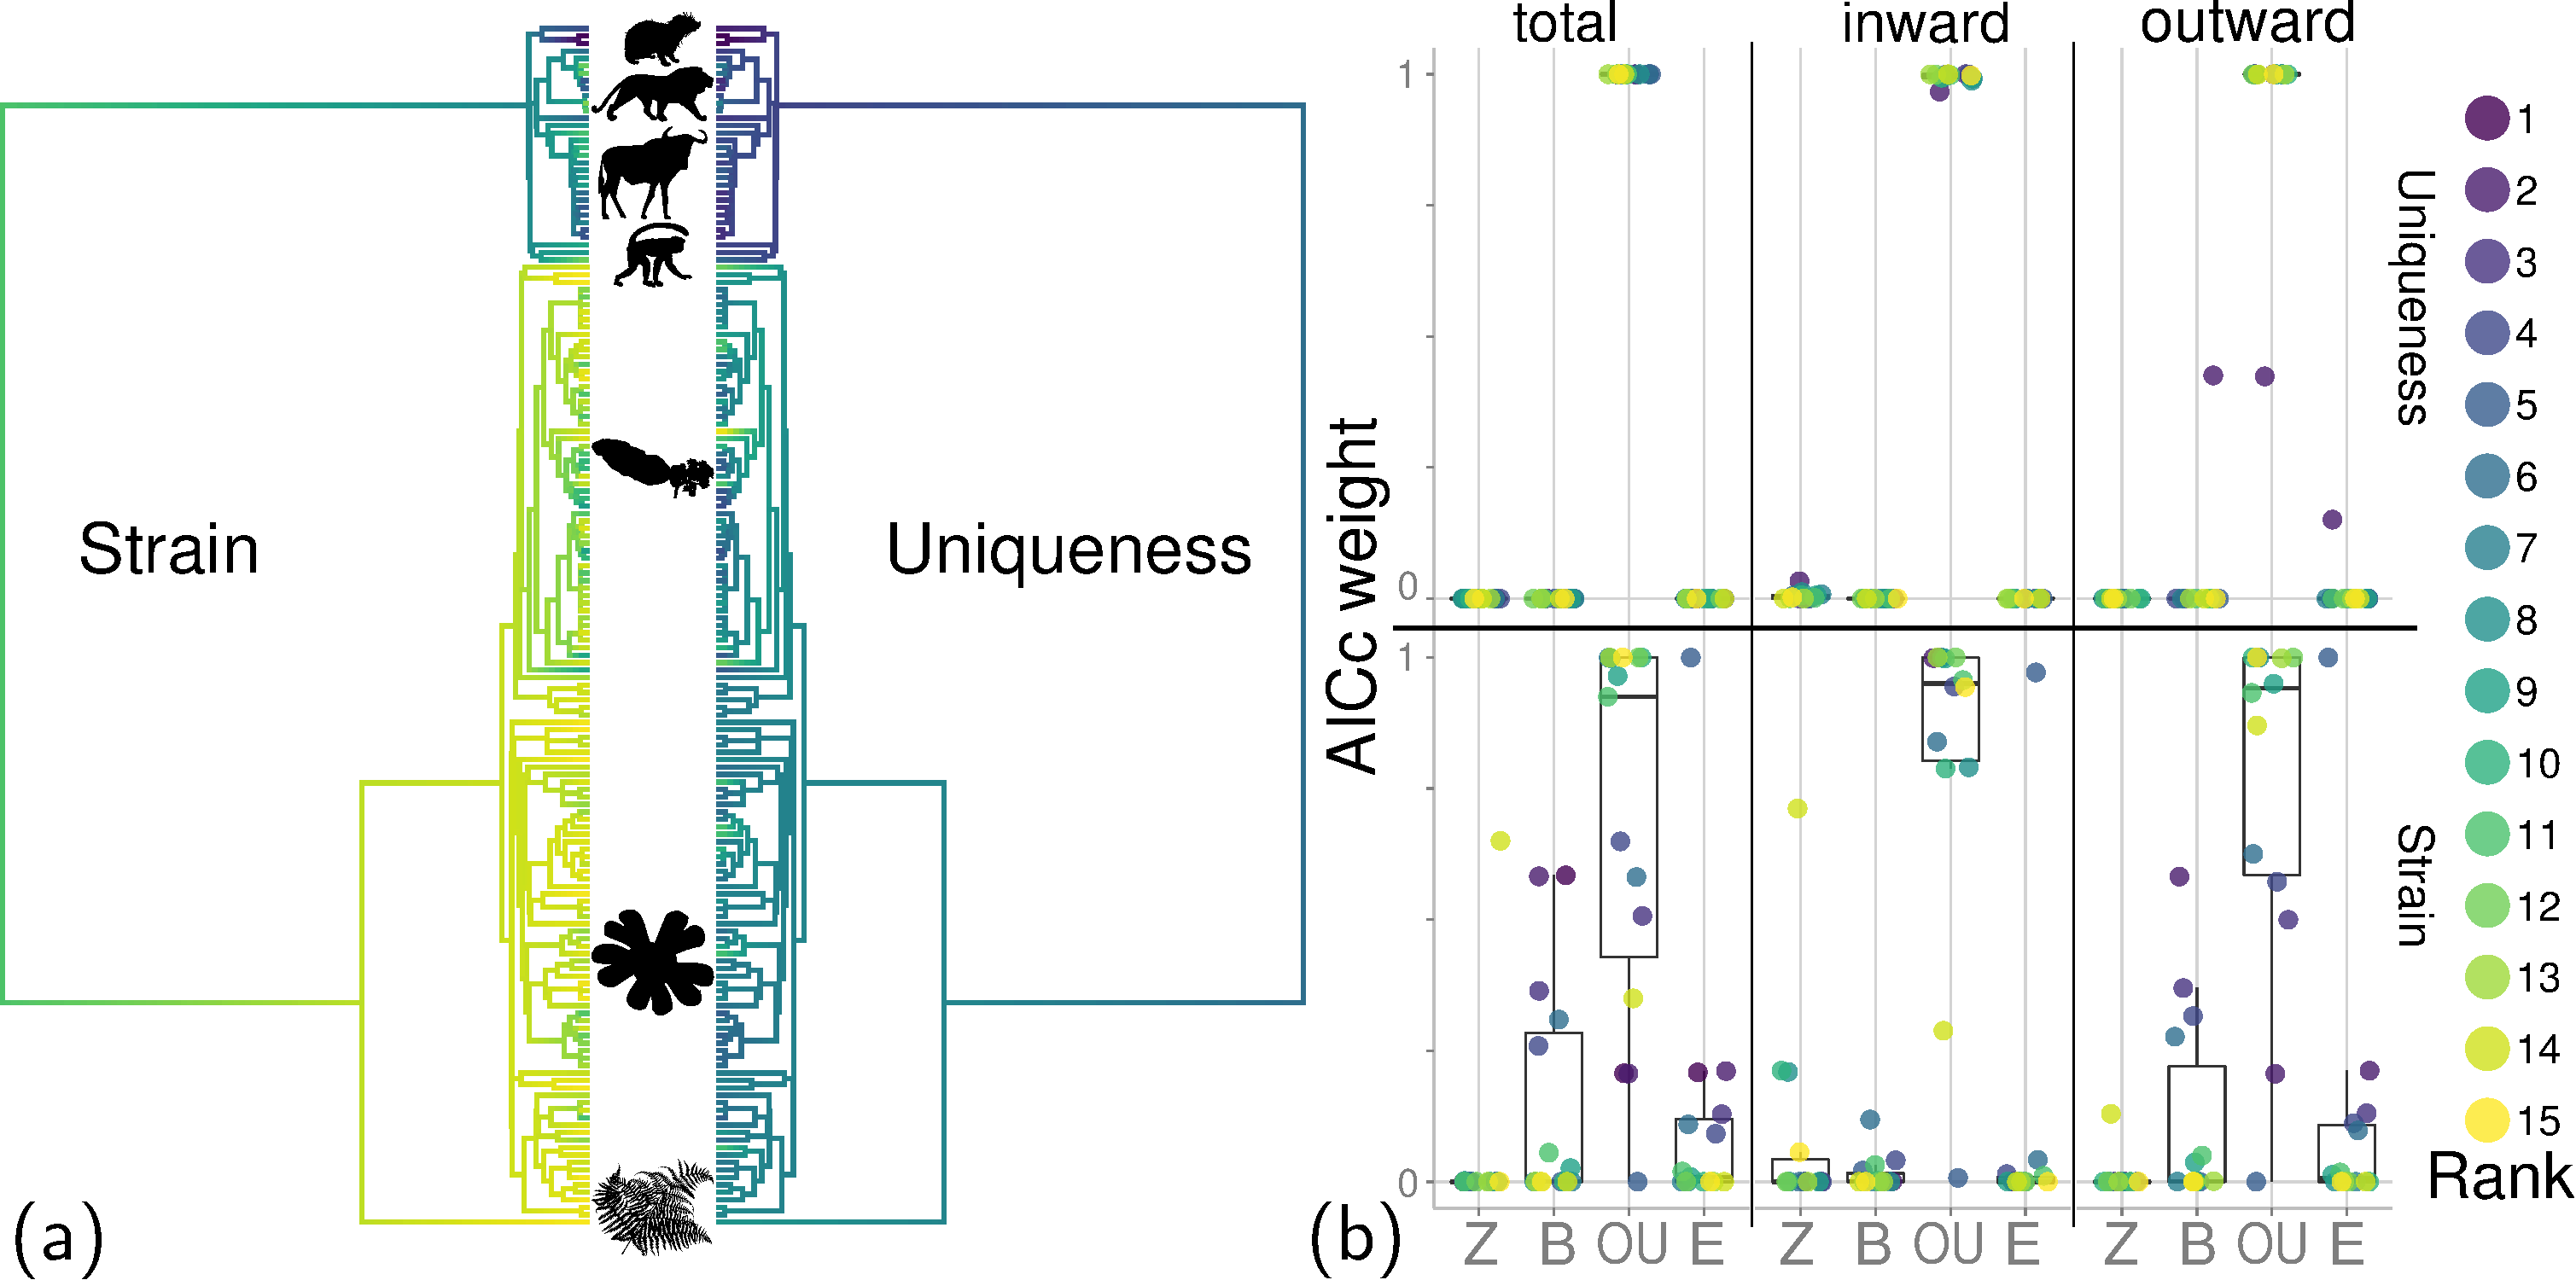
\includegraphics[width=\textwidth]{./Images/Figure_2.pdf}
\end{figure}
\newpage

\subsection*{Figure 3}
(a) There is a significant correlation between a species' uniqueness and strain for
the species as prey (outward) and as predators and prey (total). For
model dimensions $d > 3$, the correlation is not consistently
significant for the species as a predator (inward).
(b) There is a significant correlation between the species' (inward and total) strain and
uniqueness and the species' contribution to the functional diversity (the
loss of abstract functional diversity after the removal of a species). The correlation
between a species' outward strain and contribution to functional diversity is not significant for low dimensions.
The dashed red lines correspond to $p = 0.05$.

\begin{figure}[h!]
 \centering
 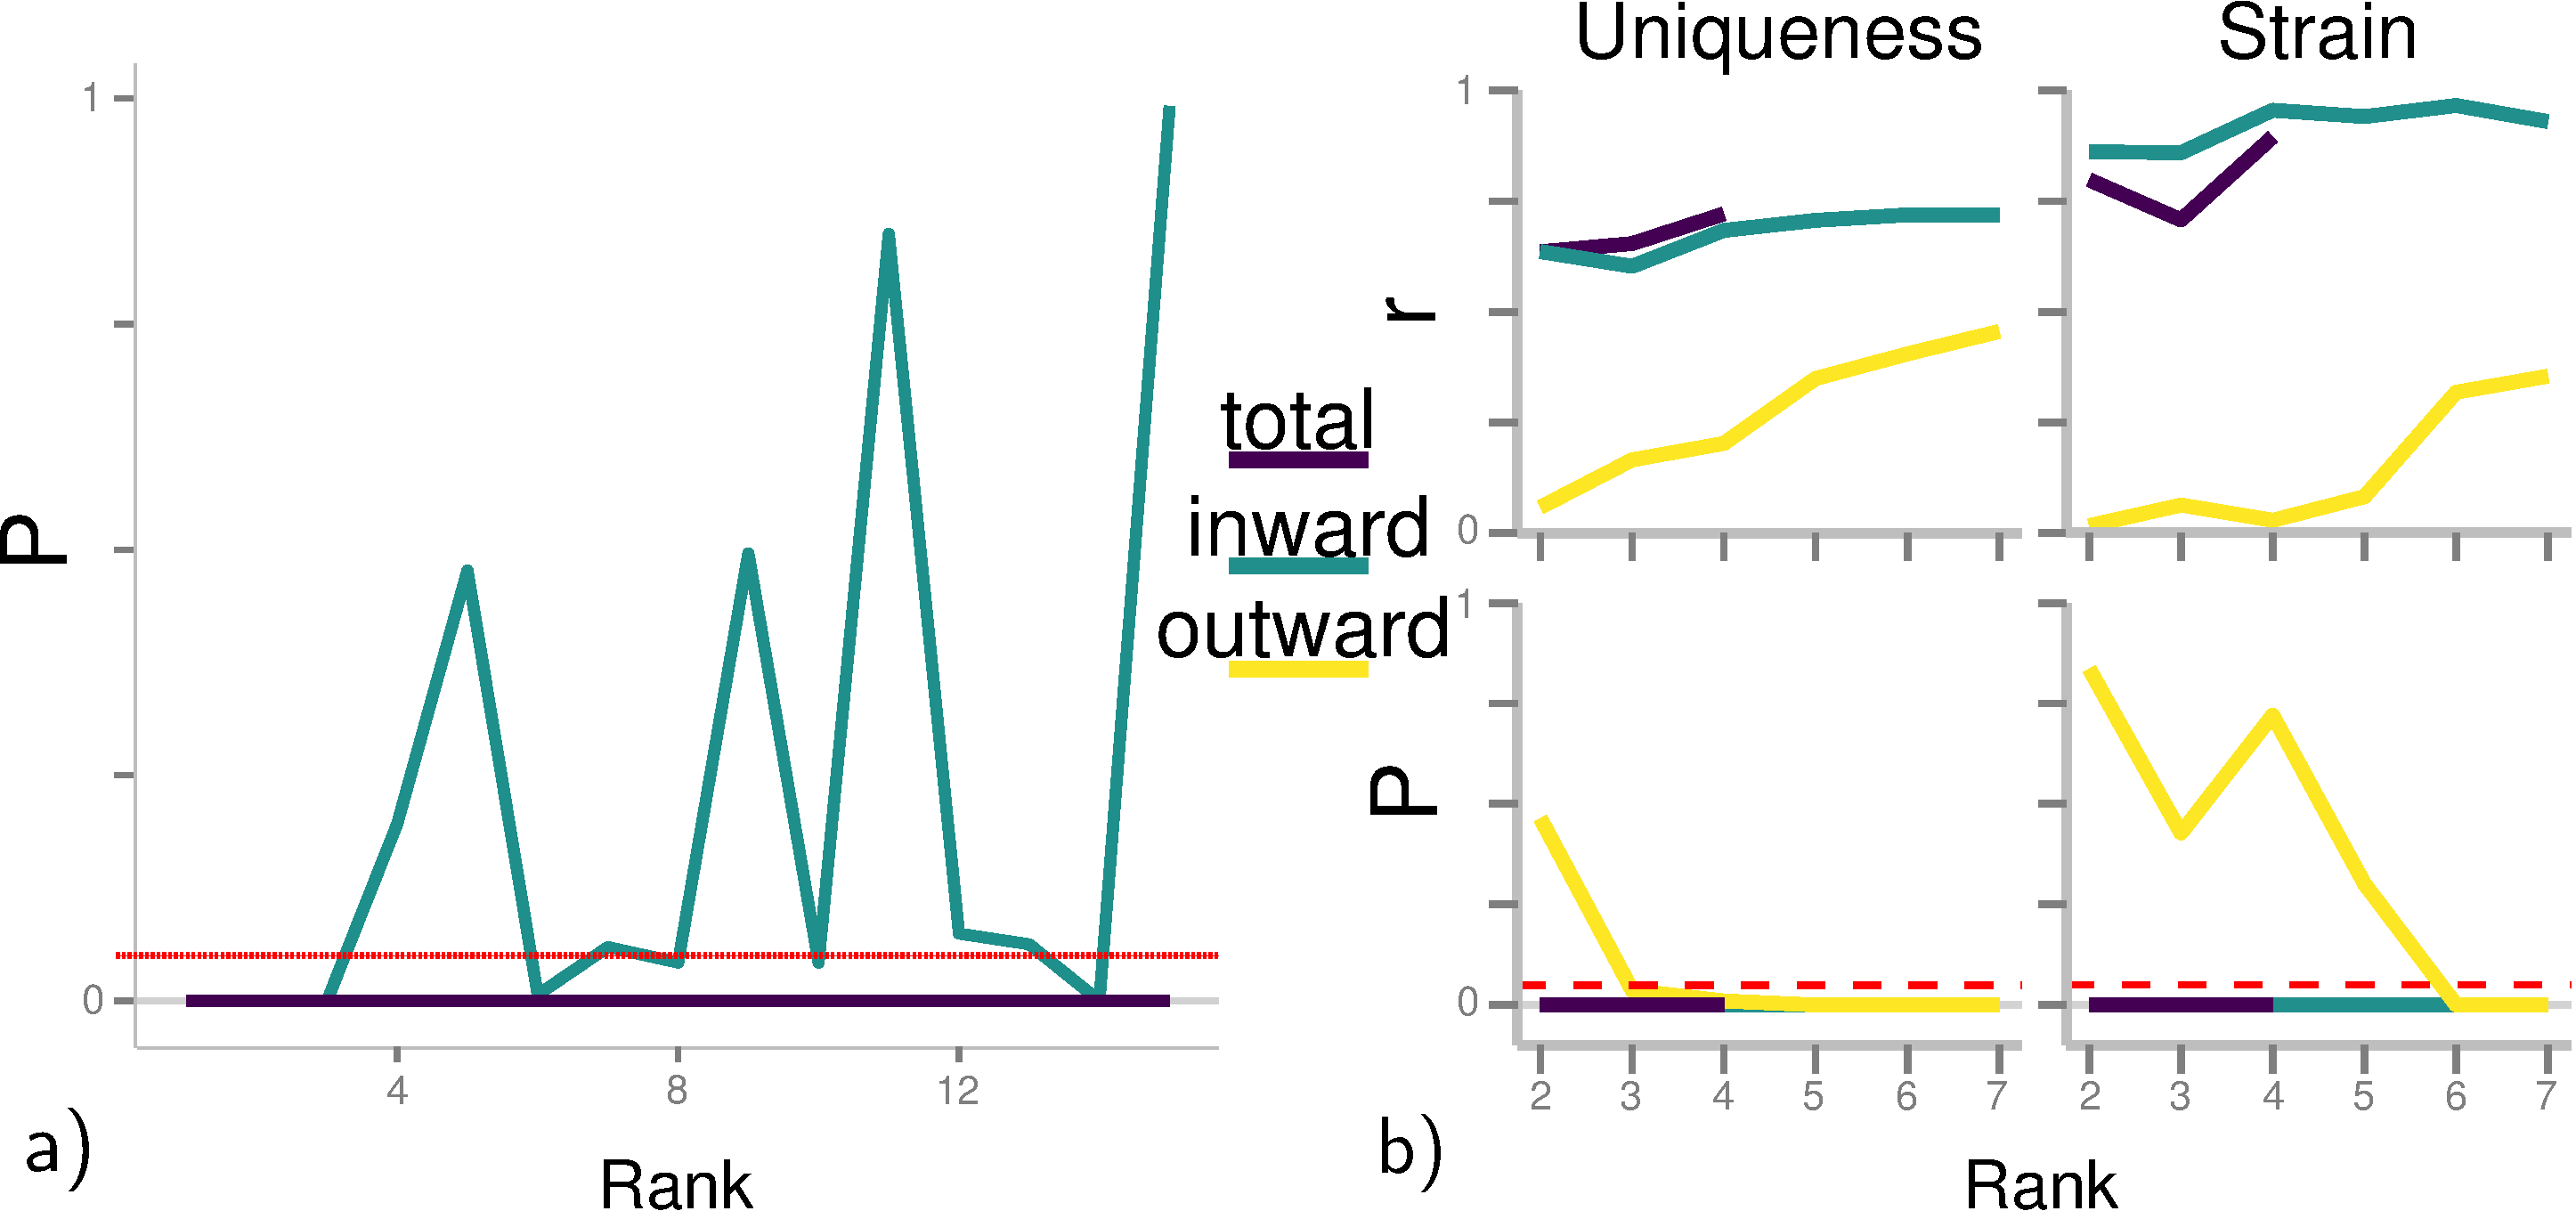
\includegraphics[width=\textwidth]{./Images/Figure_3.pdf}
\end{figure}
\newpage

\subsection*{Figure 4}
Correlation between a species' strain and uniqueness
(as a predator, inward; prey, outward; predator and prey, total)
and the species' betweenness (BC), closeness (CC), degree (DC),
eigenvector (EC), information (IC), and subgraph (SC)
centralities. Strengths and significances depend on the combination
of the centrality index (the correlation is significant for most centralities
except EC and IC), functional space (the correlation with the outward strain
and uniqueness is weak) and model dimension (the correlation is stronger
for low $d$). The dashed red lines correspond to $r = 0$ and $p = 0.05$.

\begin{figure}[h!]
 \centering
 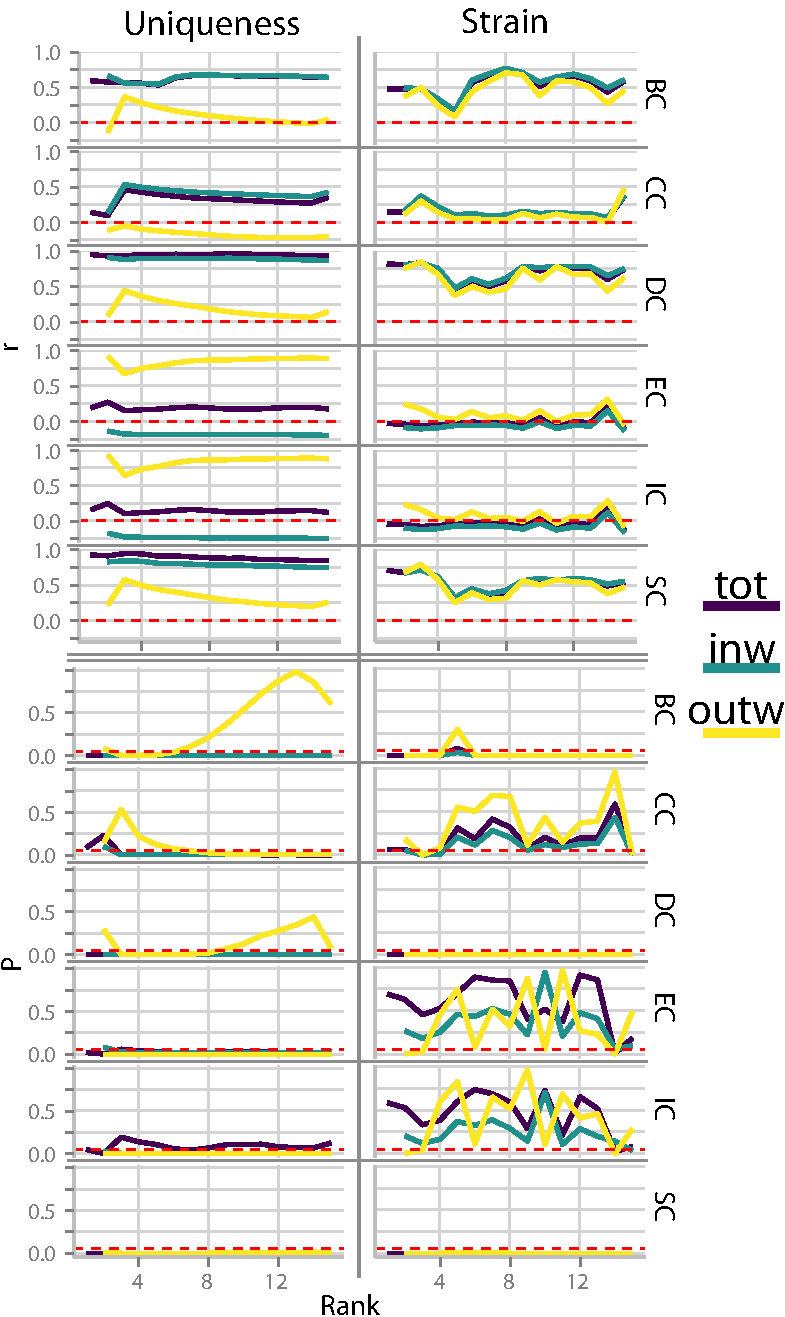
\includegraphics[height=0.6\textheight]{./Images/Figure_4.pdf}
\end{figure}
\newpage

\subsection*{Table 1}

The 10 species in the Serengeti National Park food web
\citep{baskerville2011spatial} with the highest strain (as both predators and prey)
and their ordering based on ecological uniqueness  (as both predators and
prey), contribution to functional diversity (diversity, as both predators and
prey) and equal splits (a measure of evolutionary distinctiveness). Strain,
uniqueness and contribution to functional diversity are positively correlated.
However, although there are species (e.g., the Afrotheria clade) with a high
score in all four measures, in general, there is no significant linear correlation between
ecological relevance and evolutionary distinctiveness.\newline

\begin{tabular}{|l|*{4}{c|}}
\hline
Species	&Strain	&Uniqueness	&Diversity &Equal Splits\\
\hline
\emph{Procavia capensis}	&1.32	&1	&3	&6.5\\
\emph{Heterohyrax brucei}	&0.88	&2	&1	&6.5\\
\emph{Loxodonta africana}	&0.32	&7	&6	&2\\
\emph{Panthera pardus}		&0.31	&3	&10	&148.5\\
\emph{Panthera leo}		&0.18	&6	&4	&148.5\\
\emph{Eudorcas thomsonii}	&0.17	&8	&19	&150.5\\
\emph{Nanger granti}		&0.16	&5	&13	&150.5\\
\emph{Connochaetes taurinus}	&0.15	&4	&14	&138\\
\emph{Madoqua kirkii}		&0.15	&11	&2	&100\\
\emph{Aepyceros melampus}	&0.12	&13	&0	&100\\
\hline
\end{tabular}

\end{document}
